\section{Memoria}

\subsection{Rol del Sistema Operativo}
El SO debe:
\begin{itemize}
    \item Llevar un registro de las partes de memoria que se están utilizando y de aquellas que no.
    \item Asignar espacio en memoria principal a los procesos cuando estos lo necesitan.
    \item Liberar espacio de memoria asignada a procesos que han terminado.
    \item Lograr que el programador se abstraiga de la asignación de los programas.
    \item Brindar seguridad entre los procesos para que unos no accedan a secciones privadas de otros.
    \item Brindar la posibilidad de acceso compartido a determinadas secciones de la memoria.
    \item Garantizar el rendimiento.
\end{itemize}

\subsection{Requisitos}
\begin{itemize}
    \item \textbf{Reubicación}
    \begin{itemize}
        \item El programador no debe ocuparse de conocer dónde será colocado en la memoria RAM.
        \item Mientras un proceso se ejecuta, puede ser sacado y traído a la memoria (swap) y, posiblemente, colocarse en diferentes direcciones.
        \item Las referencias a la memoria se deben "traducir" según la ubicación actual del proceso.
    \end{itemize}
    \item \textbf{Protección}
    \begin{itemize}
        \item Los procesos NO deben referenciar/acceder a direcciones de memoria de otros procesos (salvo que tengan permiso).
        \item El chequeo se debe realizar durante la ejecución.
    \end{itemize}
\item \textbf{Compartición}
    \begin{itemize}
        \item Permitir que varios procesos accedan a la misma porción de memoria.
        \item Permitir un mejor uso de la memoria principal, evitando copias innecesarias (repetidas) de instrucciones.
    \end{itemize}
\end{itemize}

\subsection{Direcciones}
\subsubsection{Espacio de direcciones}
\begin{itemize}
    \item Rango de direcciones (a memoria) posibles que un proceso puede utilizar para direccionar sus instrucciones y datos.
    \item Es independiente de la ubicación "real" del proceso en la memoria RAM.
\end{itemize}

\subsection{Tipos de direcciones}
\begin{itemize}
    \item \textbf{Lógicas/Virtuales}
    \begin{itemize}
        \item Referencia a una localidad de memoria.
        \item Representa una dirección en el "Espacio de Direcciones del Proceso".
    \end{itemize}
    \textbf{Físicas}
    \begin{itemize}
        \item Referencia una localidad en la memoria principal.
    \end{itemize}
\end{itemize}
Es necesario algún tipo de conversión de direcciones lógicas a físicas y viceversa.
\subsubsection{Conversión de Direcciones}
Una forma simple de realizar la conversión es utilizando registros auxiliares.
\begin{itemize}
    \item \textbf{Registro Base:} dirección de comienzo del Espacio de Direcciones del proceso en la memoria principal.
    \item \textbf{Registro Límite} dirección final del proceso o medida del proceso.
    \item Ambos valores se fijan cuando el espacio de direcciones del proceso es cargado a memoria.
    \item Varían entre procesos.
\end{itemize}
    Si la conversión se realiza en tiempo de ejecución, las direcciones lógicas se denominan \textbf{direcciones virtuales}, y son diferentes a las físicas.
En este caso, el mapeo entre ambos tipos de direcciones se realiza por hardware, mediante la \textbf{Memory Management Unit (MMU)}.
\begin{figure}
    \begin{center}
        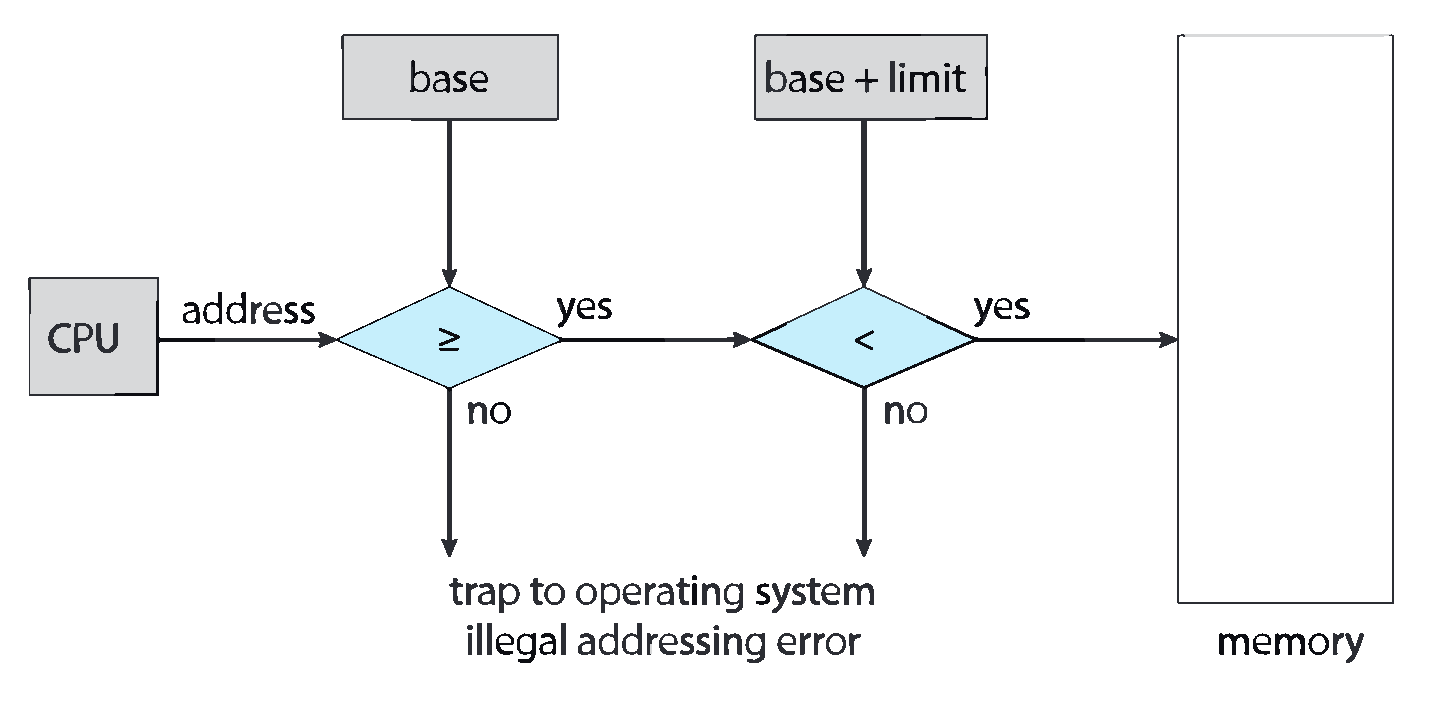
\includegraphics[width=0.75\textwidth]{assets/ConversionDirecciones.pdf}
    \end{center}
    \caption{Protección de direcciones mediante registros base y límite.}\label{fig:69}
\end{figure}
\subsection{Memory Management Unit (MMU)}
\begin{itemize}
    \item Es un dispositivo de hardware que mapea direcciones virtuales a físicas.
    \item Es parte de la CPU.
    \item Reprogramarla es una operación privilegiada.
    \item El valor en el "registro de realocación" es sumado a cada dirección generada por el proceso de usuario al momento de acceder a la memoria.
    \item Los procesos solo utilizan direcciones virtuales.
\end{itemize}
\begin{figure}[h]
    \begin{center}
        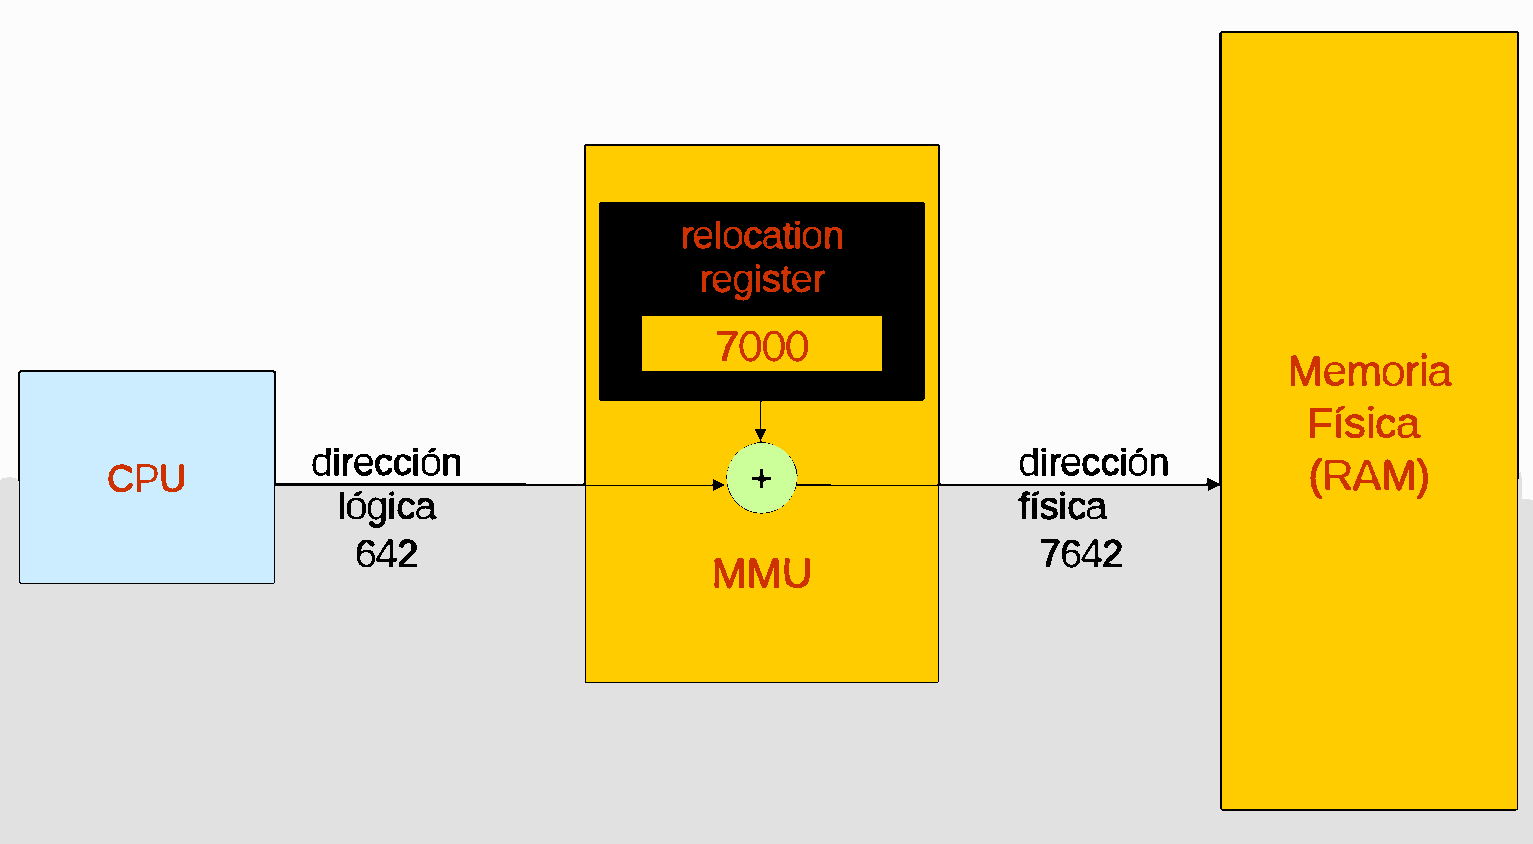
\includegraphics[width=0.70\textwidth]{assets/MMU.pdf}
    \end{center}
    \caption{Funcionamiento de la MMU}\label{fig:}
\end{figure}

\subsection{Mecanismos de asignación de memoria}
\begin{itemize}
    \item \textbf{Particiones Fijas}
    \begin{itemize}
        \item La memoria se divide en particiones o regiones de tamaño fijo (del mismo tamaño o no).
        \item Alojan un proceso cada una.
        \item Cada proceso se coloca de acuerdo a algún criterio (worst-fit, best-fit, etc).
    \end{itemize}
    \item \textbf{Particiones Dinámicas}
    \begin{itemize}
        \item Las particiones varían en tamaño y número.
        \item Alojan un proceso cada una.
        \item Cada partición se genera en forma dinámica, del tamaño exacto que necesita el proceso.
    \end{itemize}
\end{itemize}

\subsection{Fragmentación}
La \textbf{fragmentación} se produce cuando una alocalidad de memoria no puede ser utilizada por no encontrarse en forma continua.
Existen dos tipos:
\begin{itemize}
    \item \textbf{Fragmentación Interna}
    \begin{itemize}
        \item Se produce en el esquema de particiones fijas.
        \item Es la porción de la partición que queda sin utilizar.
    \end{itemize}
    \item \textbf{Fragmentación Externa}
    \begin{itemize}
        \item Se produce en el esquema de particiones dinámicas.
        \item Son huecos que van quedando en la memoria a medida que los procesos finalizan.
        \item Al no encontrarse en forma contigua, puede darse el caso de que tengamos memoria libre para alojar un proceso, pero que no la podamos utilizar.
        \item Puede solucionarse utilizando la \textbf{compactación}.
    \end{itemize}
\end{itemize}

\subsection{Paginación}
\begin{itemize}
    \item La memoria física es dividida lógicamente en pequeños trozos de igual tamaño llamados \textbf{Marcos}.
    \item La memoria lógica (espacio de direcciones) es dividida en trozos de igual tamaño que los marcos, llamados \textbf{Páginas}.
    \item El SO debe mantener una tabla de páginas por cada proceso, donde cada entrada contiene (entre otras), el Marco en el que se coloca cada página.
    \item La dirección lógica se interpreta como un número de página y un desplazamiento dentro de la misma.
\end{itemize}
\begin{figure}[h]
    \begin{center}
        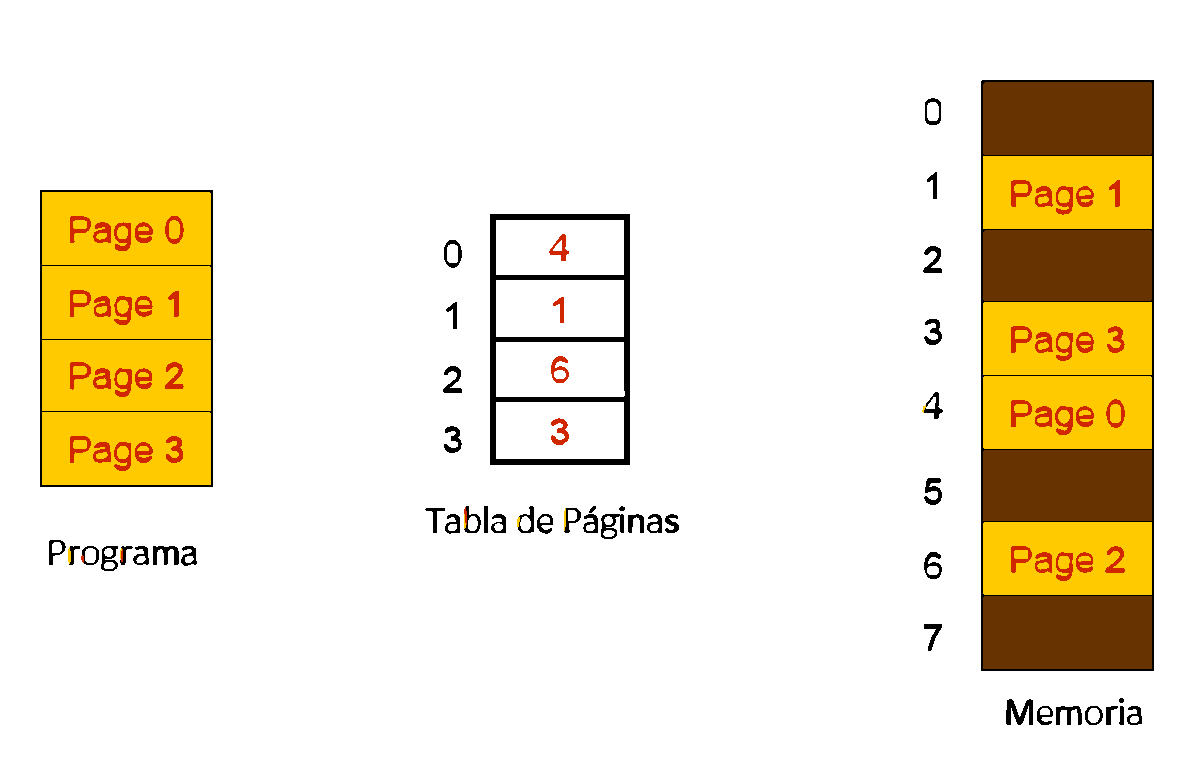
\includegraphics[width=0.70\textwidth]{assets/Paging.pdf}
        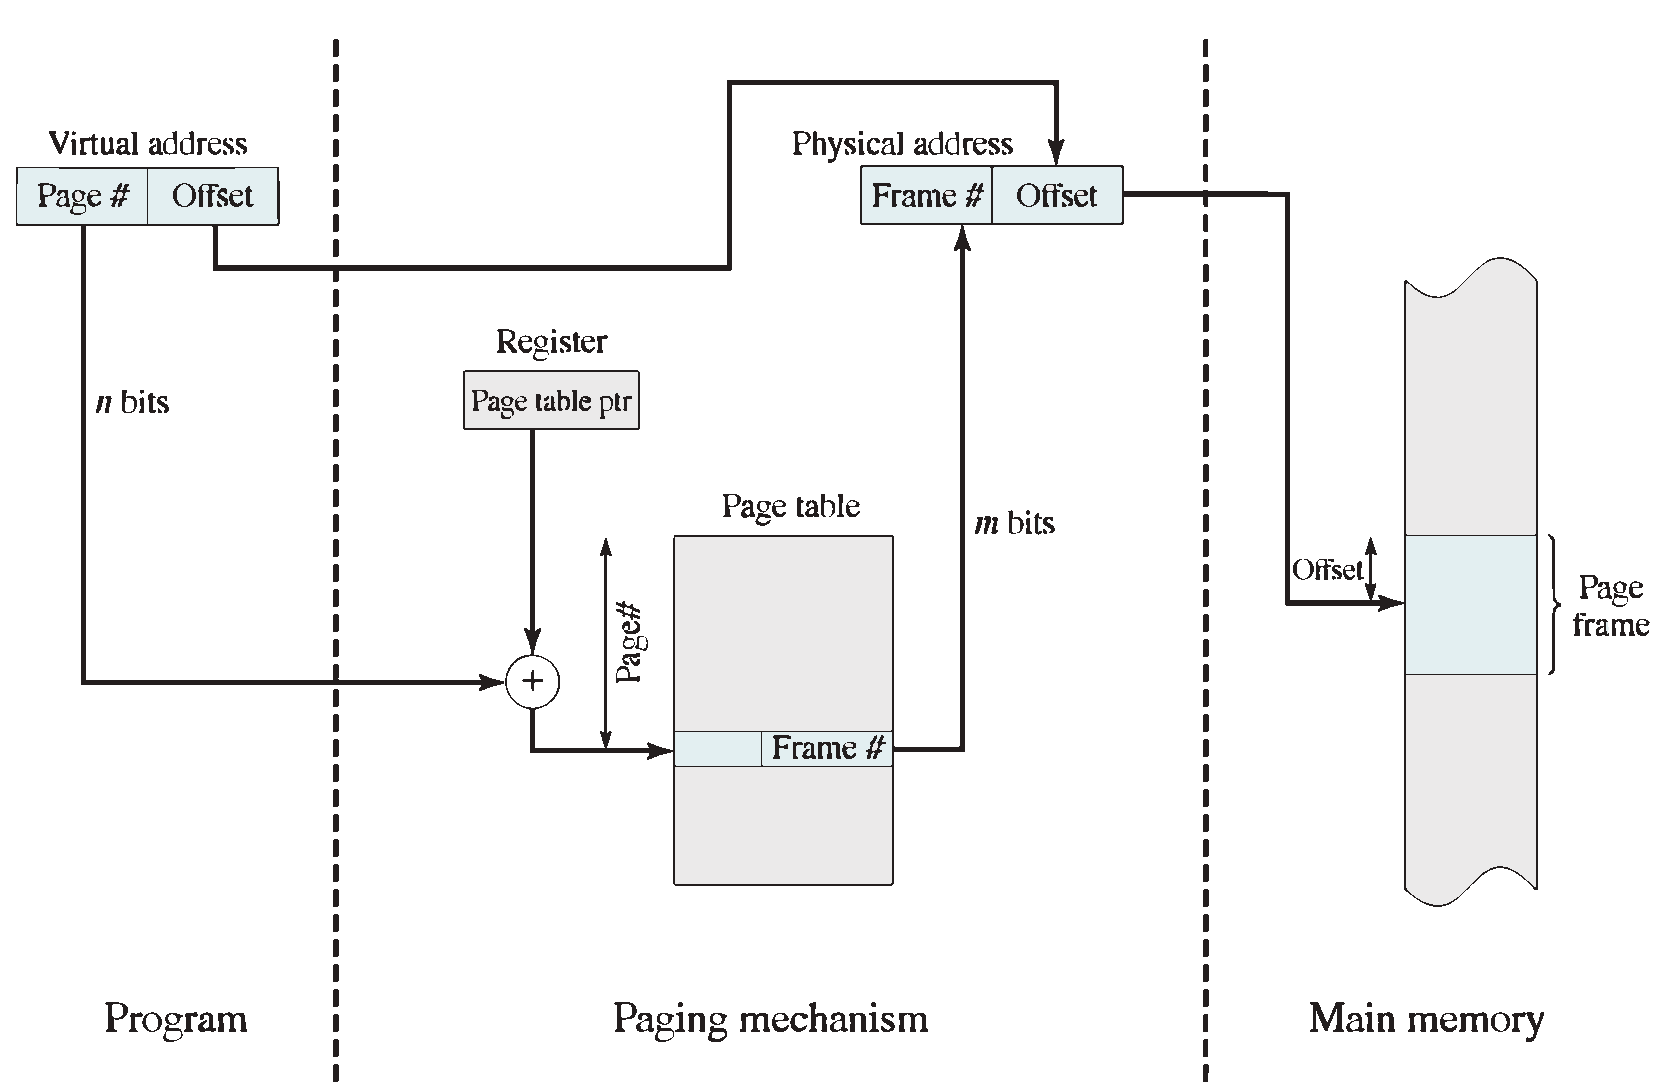
\includegraphics[width=0.80\textwidth]{assets/PagingTraslation.pdf}
    \end{center}
    \caption{Ejemplo de Paginación}\label{fig:}
\end{figure}
\pagebreak

\subsection{Segmentación}
\begin{itemize}
    \item Esquema que se asemeja a la "visión del usuario". El programa se divide en partes/secciones.
    \item Un programa es una colección de segmentos. Un segmento es una unidad lógica, como Programa Principal, Procedimientos y Funciones, variables locales/globales, etc.
    \item Puede causar fragmentación.
    \item Todos los segmentos de un programa pueden no tener el mismo tamaño.
    \item Las direcciones lógicas consisten en 2 partes:
    \begin{itemize}
        \item Selector de Segmento.
        \item Desplazamiento dentro del segmento. 
    \end{itemize}
    \item \textbf{Tabla de Segmentos:} permite mapear la dirección lógica a física. Cada entrada contiene:
    \begin{itemize}
        \item Base: Dirección física del comienzo del segmento.
        \item Límite: Tamaño del segmento.
    \end{itemize}
    \item Segment-Table base register (STBR): contiene la dirección de la tabla de segmentos.
    \item Segment-Table length register (STLR): contiene la cantidad de segmentos de un programa.
\end{itemize}
%it just works
\vspace{-0.5cm}
\begin{figure}[h]
    \begin{center}
        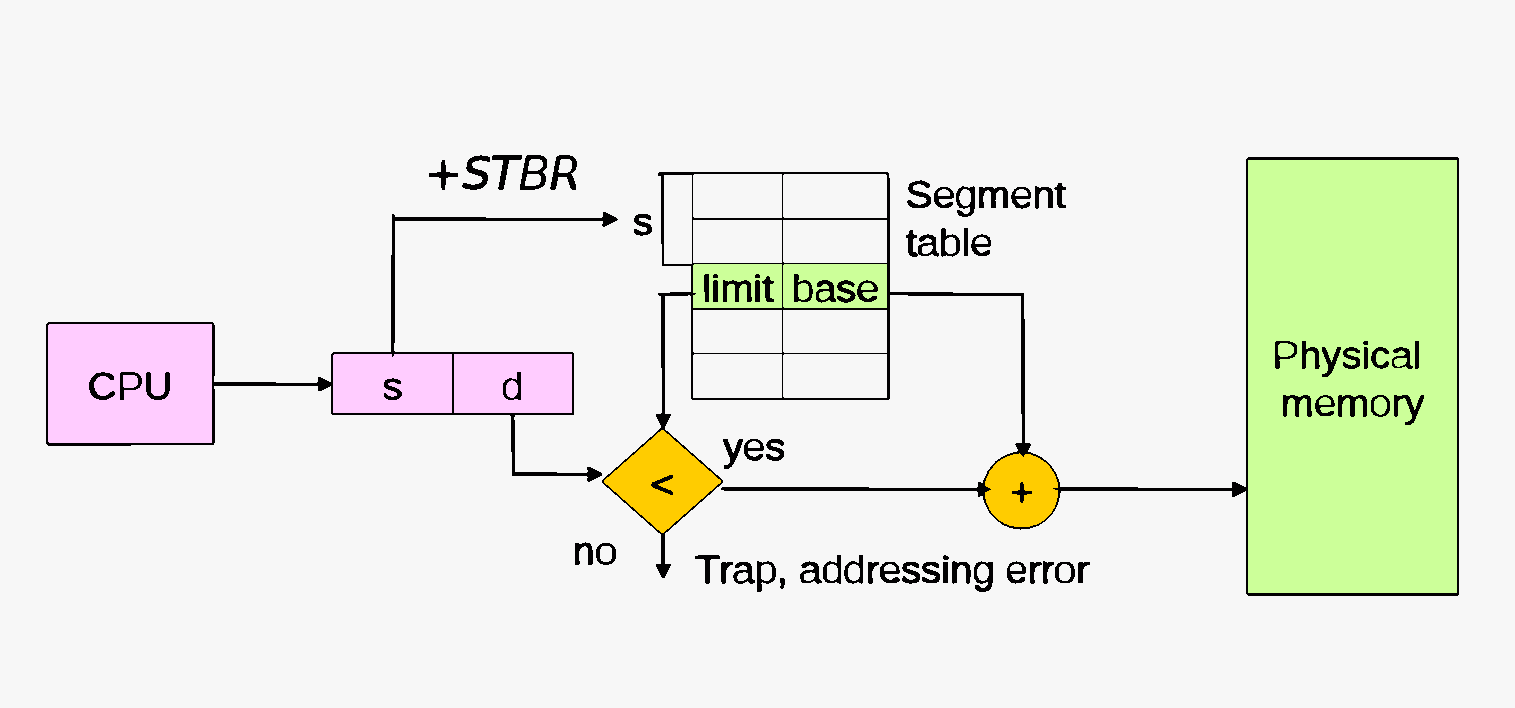
\includegraphics[width=0.90\textwidth]{assets/SegmentationTranslation.pdf}
    \end{center}
    \caption{Traducción de direcciones en un sistema con Segmentación}\label{fig:}
\end{figure}
\pagebreak
\subsubsection{Segmentación Paginada}
\begin{itemize}
    \item La paginación:
    \begin{itemize}
        \item Transparente al programador.
        \item Elimina Fragmentación Externa.
    \end{itemize}
    \item La segmentación:
    \begin{itemize}
        \item Es visible al programador.
        \item Facilita modularidad, estructuras de datos grandes y da mejor soporte a la compartición y protección.
    \end{itemize}
    \item \textbf{Segmentación Paginada:} cada segmento es dividido en páginas de tamaño fijo.
\end{itemize}
\begin{figure}[h]
    \begin{center}
        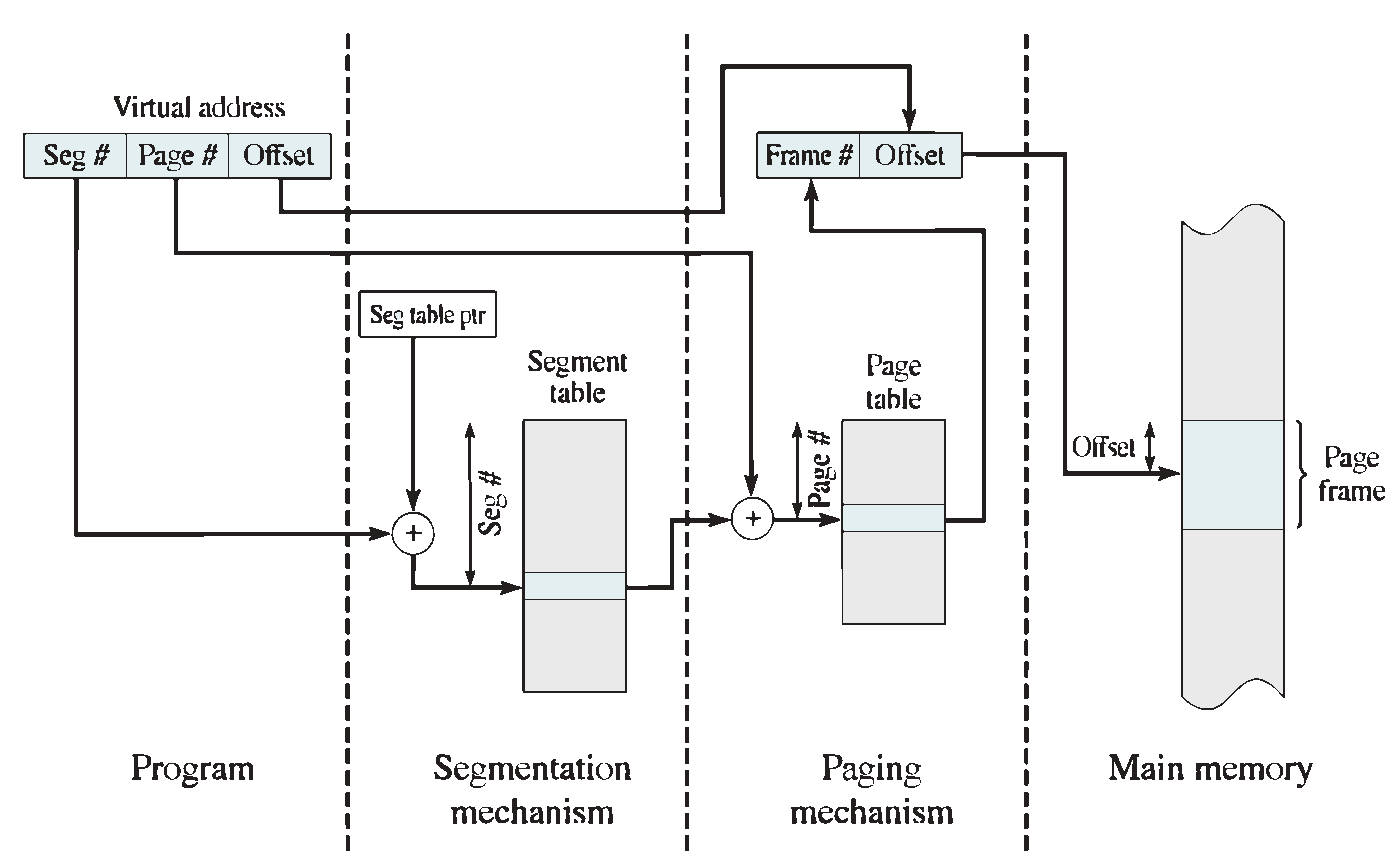
\includegraphics[width=0.95\textwidth]{assets/SegmentacionPaginada.pdf}
    \end{center}
    \caption{Traducción de direcciones en un sistema con Segmentacion Paginada}\label{fig:}
\end{figure}
